\section{Introduction}
% Logs are important. (But they can be forked breaking security guarantees of the apps using them. For example, CT logs. Recent work looks to Bitcoin due to its inherent resilience to forks. However, recent work is not efficient. Here we show how to do it efficiently.)
% ------------------
Security often depends on \emph{non-equivocation}\cite{frientegrity,coniks}.
For example, when a Certificate Authority (CA) equivocates by signing contradicting certificates for the same identity, it can impersonate websites and compromise users' privacy.
In fact, this has happened many times in the past\cite{cahacksurvey,cafrance,cahacks,caturkey,etisalat,mitmgoogle,certifiedlies}.
To prevent equivocation, Certificate Transparency (CT)\cite{ct} has been introduced as a way of publicly logging all CA-issued certificates.
However, a CT log server can still equivocate about the log of issued certificates and, together with a colluding CA, can launch impersonation attacks.
While gossiping\cite{ctgossip} about the log can help detect equivocation, detection can be slow or not happen at all, as gossip messages can be delayed indefinitely.
Another example is the Tor\cite{tor} anonymity network, where malicious directory servers can equivocate about the set of Tor relays and deanonymize users by tricking them to use malicious relays\cite{tortransparency}.
Thus, we believe non-equivocation is an important security requirement in many systems today, such as public-key distribution, blockchain-based transparency\cite{keybase,blockstack} and software transparency (see \secref{sec:background:motivation}).

% Fork-consistency is not enough
% ------------------------------
Unfortunately, without online trusted parties, achieving non\hyp{}equivocation is impossible\cite{sundrosdi}.
To deal with this impossibility result, systems resort to enforcing a weaker property called \emph{fork consistency}\cite{sundrosdi}.
Fork-consistent systems essentially make equivocation ``permanent'' and thus easier to prove later when clients are able to communicate or ``gossip'' out-of-band.
However, as illustrated above, for systems such as \pkds and Tor directory servers, undetected equivocation attacks can seriously impact users' security.
Thus, we believe a more proactive approach\cite{cosi} to security is desirable for such systems.

% Bitcoin witnessing is promising
% -------------------------------
To prevent equivocation proactively, recent work\cite{keybase,blockstack} uses the Bitcoin blockchain\cite{bitcoin}, as a witness.
We believe this \emph{Bitcoin witnessing} approach, though currently inefficient, is promising for three reasons.
First, this approach makes equivocation as hard as forking the Bitcoin blockchain itself, which has proven resistant to forking attacks.
Second, this approach only relies on a single global witness, namely the Bitcoin blockchain, obviating the need for users to obtain correct cryptographic identities of multiple trusted entities, such as log providers and auditors as in CT\cite{ct}, or witnesses as in CoSi\cite{cosi}.
It also has the advantage of not requiring the witness to keep any secrets, which if compromised would result in equivocation.
Third, the Bitcoin blockchain's open, decentralized and censorship-resistant nature makes deployment of witnessing schemes easy and interference with them hard.
Unfortunately, the main drawback of existing Bitcoin witnessing schemes has been that auditors have to download the entire Bitcoin blockchain, which, in November 2016, was almost \blockchainsize\cite{bitcoin-size} in size and growing by 52 GB every year.

% or t for top, b for bottom, h for here (https://tex.stackexchange.com/questions/35125/how-to-use-the-placement-options-t-h-with-figures)
\begin{figure}[t]
  \centering
    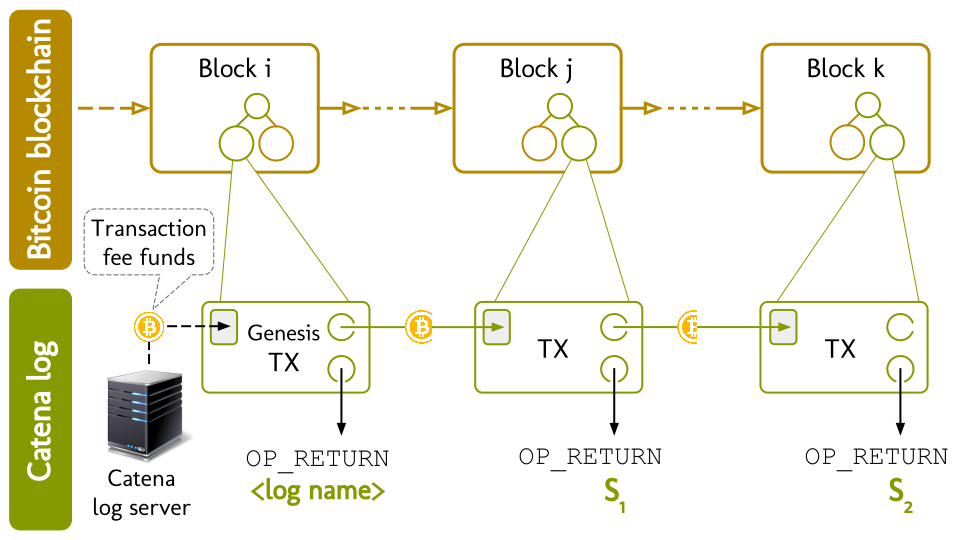
\includegraphics[width=1\columnwidth]{figs/overview.eps}
    \vspace{-.5cm}
    \caption{A \Sys log is a chain of Bitcoin transactions. Each \Sys transaction has two outputs: (1) a continuation output, which is spent by the next \Sys transaction, thus creating a chain and (2) an \opret output, which commits some application-specific statement. The server pays Bitcoin transaction fees for each issued statement. For applications that publish statements often, batching can be used to keep the fee per statement low.}
    \label{fig:catena-overview}
\end{figure}

% Elevator pitch
% --------------
This paper presents \emph{\Sys}, an efficient Bitcoin-based witnessing scheme that dramatically reduces auditors' bandwidth overhead.
At a high level, \Sys is a tamper-evident log\cite{ht} built on top of the Bitcoin blockchain.
\Sys prevents adversarial log servers who cannot fork the Bitcoin blockchain from equivocating about a log of application-specific statements.
Importantly, auditors who run \Sys clients can check the log for non-equivocation efficiently via Simplified Payment Verification (SPV)\cite{bitcoin} (see \secref{sec:background:bitcoin:thin}). 
This drastically decreases auditing bandwidth from \blockchainsize\cite{bitcoin-size} to only tens of megabytes, as \Sys clients only need to download Bitcoin block headers and small Merkle proofs under some of those headers.
Furthermore, after all block headers are downloaded, the bandwidth decreases to less than 1 KB of data every 10 minutes.


\subsection{Efficient Non-equivocation via Bitcoin}

Previous Bitcoin witnessing schemes\cite{keybase,blockstack} cannot \emph{efficiently} prove non-membership of inconsistent statements unless auditors download all the transactions in the Bitcoin blockchain.
Our design addresses this issue by allowing \Sys clients to skip downloading all irrelevant transactions while still guaranteeing non-equivocation.
\emph{The key idea behind \Sys is that Bitcoin's mechanism for preventing double spends can actually be regarded as a non-membership proof.}
Specifically, Bitcoin proves that no transactions double spending a previous transaction's output exist.
That is, if a client verifies blockchain membership for a transaction $tx_2$ which spends a previous transaction output $tx_1[0]$, that client has also implicitly verified that no other transaction $tx_2'$ which spends $tx_1[0]$ exists in the blockchain. ($tx_1[0]$ refers to the first output of transaction $tx_1$; see \secref{sec:background:bitcoin:transactions} for Bitcoin background.)

\Sys turns this idea into a non-equivocation scheme.
Each \emph{\Sys transaction} stores exactly one statement and spends the previous \Sys transaction, creating a chain of statements as shown in \figref{fig:catena-overview}.
This implies that if an auditor sees a statement $s_i$ in the blockchain whose transaction correctly spends the transaction for the previous statement $s_{i-1}$, then \emph{that constitutes a non-membership proof that no other inconsistent statement $s_i'$ exists}.
Looked at differently, if an adversarial log server wants to equivocate about $s_i$, it has to double spend the previous \Sys transaction for $s_{i-1}$, which can only be done by forking the Bitcoin blockchain.

\subsubsection{Root-of-Trust}
\Sys guarantees that once a client correctly obtains a log's \emph{genesis transaction}, the server cannot equivocate about that log unless it forks the Bitcoin blockchain.
The genesis transaction is the first transaction in the log and acts as the root-of-trust or ``\pk'' for a \Sys log (see \secref{sec:catena:design:genesis}).
Once clients obtain the correct genesis transaction they can efficiently verify that every issued statement comes from a transaction that spends coins originating from the genesis transaction.
In \secref{sec:catena:design}, we explain how this implicitly prevents equivocation in a \Sys log.
Our design is simple and efficient and obviates the need for log servers and clients to download the full Bitcoin blockchain while ensuring the consistency of the log.

\subsubsection{Bitcoin-friendly}
% Blockstack burns funds using a ``burn address.'' Not sure why they don't simply send the coins to the OP_RETURN output which commits their data.
To embed log statements in Bitcoin transactions, \Sys uses provably-unspendable \opret transaction outputs\cite{opreturn}, which, unlike previous work\cite{keybase-opret,blockstack}, does not harm Bitcoin by polluting the unspent transaction output (UTXO) set on Bitcoin nodes.
However, we emphasize that \Sys's novelty is not in leveraging \opret (previous work already does that; see \secref{sec:related-work}), but in chaining together \opret transactions that contain log statements, which makes it possible to check for non-equivocation efficiently.
Furthermore, \Sys does not place unnecessary stress on the Bitcoin P2P network.
First, clients query the \Sys log server directly to discover statements instead of using disk-intensive Bloom filtering on the Bitcoin P2P network (see \secref{sec:background:bitcoin:thin}).
Second, to avoid depleting the small connection pool of Bitcoin's P2P network, clients query a \emph{header relay network} (HRN) to obtain the latest Bitcoin block headers (see \secref{sec:catena:design:header-relay}).
Put simply, the HRN can be thought of as an ``extension'' of Bitcoin's P2P network for handling additional block header requests coming from \Sys clients.
We discuss potential attacks on the HRN in \secref{sec:attacks:hrn}.

\subsubsection{Applications}
Due to Bitcoin's 10-minute block rate, the \Sys log server can only issue a statement every 10 minutes while clients have to wait at least 60 minutes before accepting an issued statement.
Still, even with these delays, we believe \Sys can help secure applications such as key transparency schemes, Tor directory servers and software transparency schemes.
We discuss these applications in more detail in \secref{sec:background:motivation} and discuss \Sys's application-agnostic nature in \secref{sec:discussion:agnostic}.

\subsubsection{Evaluation}
To demonstrate the feasibility of \Sys, we implement a small-scale prototype in 3000 lines of Java using the bitcoinj Simplified Payment Verification (SPV) library\cite{bitcoinj} (see \secref{sec:prototype}).
Our current prototype does not include a Header Relay Network (HRN) so it will not scale to too many \Sys clients without stressing Bitcoin's P2P network.
We leave this to future work.
We also analyze the Bitcoin transaction fees the server has to pay per issued statement and show they could be anywhere between 7 to 12 US cents per statement.
Since existing systems like Keybase\cite{keybase} already pay close to 7 US cents per transaction, we believe this cost is practical.
Finally, we use our prototype to add Bitcoin witnessing to CONIKS\cite{coniks}, a recent key transparency scheme (see \secref{sec:prototype:coniks}), to demonstrate the ease of using \Sys.


\subsection{Contributions and Organization}

To summarize, this paper makes the following contributions:
\begin{itemize}
\item A new, \emph{efficient} approach to transparency based on witnessing in the Bitcoin blockchain.
\item \Sys, an append-only log built on top of Bitcoin that is efficiently verifiable by thin clients, obviating the need to download the full Bitcoin blockchain.
\item A prototype implementation of \Sys in Java that can be used by applications today.
\end{itemize}

\heading{Organization.} We motivate \Sys and present the Bitcoin background necessary to understand our design in \secref{sec:background}. We describe our system's actors, threat model and goals in \secref{sec:model}. We present \Sys's design in \secref{sec:catena:design} and we discuss attacks and countermeasures in \secref{sec:attacks}. We discuss our prototype implementation, its overheads and our extension of CONIKS in \secref{sec:prototype}.
We discuss remaining issues and future work in \secref{sec:discussion}.
We go over related work in \secref{sec:related-work} and we conclude in \secref{sec:conclusion}.
